\documentclass[12pt]{article}
\usepackage[utf8]{inputenc}

\usepackage{enumitem}
\usepackage[margin=2cm]{geometry}

\usepackage{amsmath, amsfonts, amssymb}
\usepackage{graphicx}
\usepackage{tikz}
\usepackage{pgfplots}
\usepackage{multicol}

\usepackage{comment}
\usepackage{url}
\usepackage{calc}
\usepackage{subcaption}

\usepackage{array}

\setlength\parindent{0pt}

\usepackage{fancyhdr}
\pagestyle{fancy}
\fancyhf{}
\renewcommand{\headrulewidth}{2pt}
\renewcommand{\footrulewidth}{0pt}
\rfoot{\thepage}
\lhead{\textsc{Math} 244}
\chead{\textsc{Homework 3}}
\rhead{Fall 2023}

\pgfplotsset{compat=1.16}

% MATH commands
\newcommand{\ga}{\left\langle}
\newcommand{\da}{\right\rangle}
\newcommand{\oa}{\left\lbrace}
\newcommand{\fa}{\right\rbrace}
\newcommand{\oc}{\left[}
\newcommand{\fc}{\right]}
\newcommand{\op}{\left(}
\newcommand{\fp}{\right)}

\newcommand{\bi}{\mathbf{i}}
\newcommand{\bj}{\mathbf{j}}
\newcommand{\bk}{\mathbf{k}}
\newcommand{\bF}{\mathbf{F}}

\newcommand{\ra}{\rightarrow}
\newcommand{\Ra}{\Rightarrow}

\newcommand{\sech}{\mathrm{sech}\,}
\newcommand{\csch}{\mathrm{csch}\,}
\newcommand{\curl}{\mathrm{curl}\,}
\newcommand{\dive}{\mathrm{div}\,}

\newcommand{\ve}{\varepsilon}
\newcommand{\spc}{\vspace*{0.5cm}}

\DeclareMathOperator{\Ran}{Ran}
\DeclareMathOperator{\Dom}{Dom}

\newcommand{\exo}[3]{\noindent\textcolor{red}{\fbox{\textbf{Section {#1}, Problem {#2}}}\hrulefill   \textbf{({#3} Pts})}\vspace*{10pt}}

\begin{document}
\thispagestyle{empty}
	\noindent \hrulefill \newline
	MATH-244 \hfill Pierre-Olivier Paris{\'e}\newline
	Homework 3 Solutions \hfill Fall 2023\newline \vspace*{-0.7cm}
	
	\noindent\hrulefill
	
	\spc
	
	\exo{15.3}{8}{10}

	A picture of the region is presented below.
	\begin{center}
	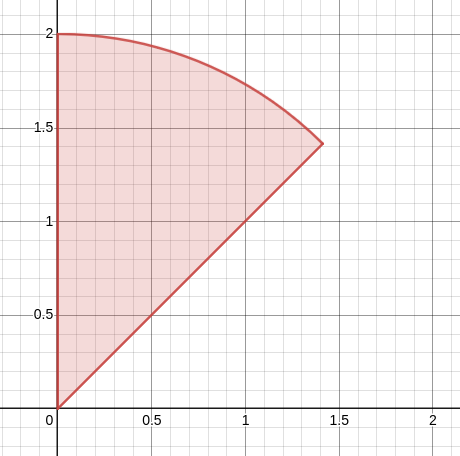
\includegraphics[scale=0.5]{domainExo8.png}
	\end{center}

	Using polar coordinates, the equation of the circle $x^2 + y^2 = 4$ becomes $r = 2$. Therefore, $0 \leq r \leq 2$. The equations $y = x$ and $x = 0$ will be used to find the bounds on the angle. When $y = x$, we then have $r \sin \theta = r \cos \theta$, so that $\tan \theta = 1$. Therefore, $\theta_1 = \pi /4$. When $x = 0$, we then have $r \cos \theta = 0$, so that $\cos \theta = 0$. Therefore, $\theta_2 = \frac{\pi}{2}$. The region, in polar coordinates, is therefore
		\begin{align*}
		R = \{ (r, \theta) \, : \, 0 \leq r \leq 2 \text{ and } \frac{\pi}{4} \leq \theta \leq \frac{\pi}{2} \} .
		\end{align*} 

	The integral in polar coordinates turns out to be
		\begin{align*}
		\iint_R (2x - y) \, dA &= \int_{\pi/4}^{\pi/2} \int_0^2  (2r \cos \theta - r \sin \theta ) r \, dr d\theta \\
		&= \int_{\pi/4}^{\pi/2} \int_0^2 2r^2 \cos \theta - r^2 \sin \theta \, dr d\theta .
		\end{align*}
	We can now evaluate the iterated integrals:
	\begin{align*}
		\iint_R (2x - y) \, dA &= \int_{\pi/4}^{\pi/2} \left. \Big( 2\frac{r^3}{3} \cos \theta - \frac{r^3}{3} \sin \theta \Big) \right|_0^2 \, d\theta\\
		&= \int_{\pi/4}^{\pi/2} \Big( \frac{16}{3} \cos \theta - \frac{8}{3}\sin \theta \Big) \, d\theta \\
		&= \frac{8}{3} \left. (2\sin \theta + \cos \theta ) \right|_{\pi/4}^{\pi/2} \\
		%&= \frac{8}{3} \Big( (2 + 0) - \Big( \sqrt{2} + \frac{\sqrt{2}}{2} \Big) \Big) \\
		%&= \frac{8 (4 - 3\sqrt{2})}{6} \\
		&= \frac{16}{3} - 4 \sqrt{2} . \tag*{$\triangle$}
		\end{align*} .
	
	\exo{15.3}{14}{10}

	\begin{comment}
	The first equation in polar coordinates is simply $r = 2$. The second equation in polar coordinates is
		\begin{align*}
		x^2 + y^2 = 2x \iff r^2 = 2 r \cos \theta \iff r = 2 \cos \theta .
		\end{align*} 
	This second equation is a circle. The region is therefore bounded by the line $x = 0$, the circle $r = 2$, and the second circle $r = 2 \cos \theta$. The region $R$ is shown in red in the picture below.
	\begin{center}
	\includegraphics[scale=0.5]{domainExo14.png}
	\end{center}
	We see from the picture that
		\begin{align*}
		R = \{ (r, \theta ) \, : \, 0 \leq \theta \leq \pi / 2 \text{ and } 2 \cos \theta \leq r \leq 2 \} .
		\end{align*} 

	The expression of the double integral in polar coordinates is therefore
		\begin{align*}
		\iint_R x \, dA &= \int_0^{\pi /2} \int_{2 \cos \theta}^2 r \cos \theta r \, dr d\theta \\
		&= \int_0^{\pi/2} \left. \frac{r^3}{3} \right|_{2 \cos \theta}^2 \cos \theta \, d\theta \\
		&= \int_0^{\pi/2} \frac{8}{3} (\cos \theta - \cos^4 \theta ) \, d\theta \\
		&= \frac{8}{3} \left. \Big( \sin \theta - \frac{3\theta}{8} - \frac{\sin (2 \theta)}{4} - \frac{\sin (4\theta)}{32} \Big) \right|_0^{\pi/2} \\
		&= \frac{8}{3} - \frac{\pi}{2} . \tag*{$\triangle$}
		\end{align*}

	\exo{15.3}{18}{10}

	The intersection between the cardioid and the circle is found by equating their equations and finding $\theta$:
		\begin{align*}
		1 + \cos \theta = 3 \cos \theta \iff \frac{1}{2} = \cos \theta \iff \theta = \pi/3 \text{ or } \theta = -\pi/3 .
		\end{align*} 
	The region $D$ is illustrated in the picture below:
		\begin{center}
		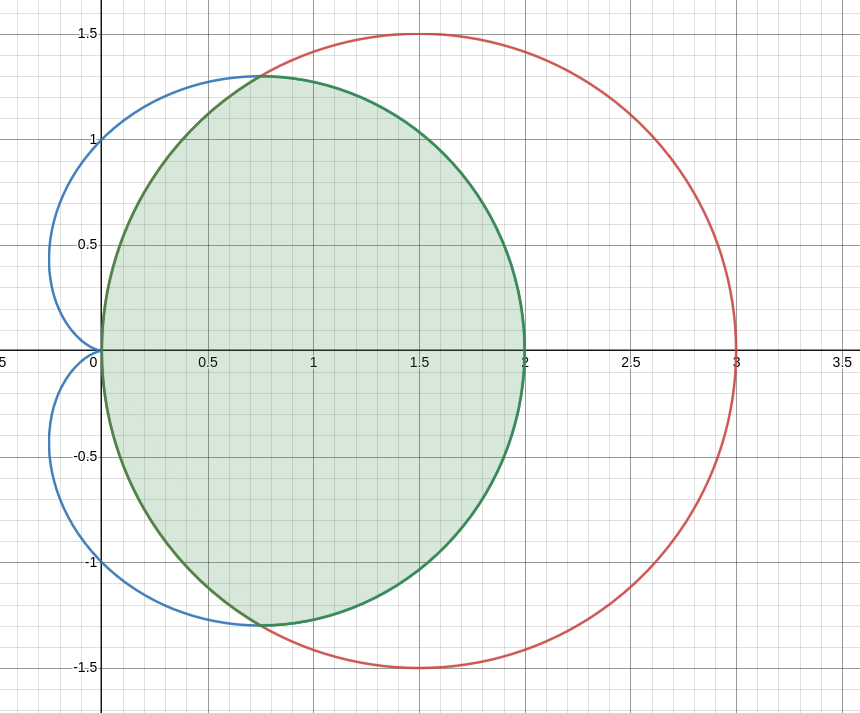
\includegraphics[scale=0.2]{exo18Hw3.png}
		\end{center}
	We see that it is symmetric about the $y = 0$ axis, so we can only compute the area of the region above the $x$-axis, and then multiply by two the result. Denote the upper half of the region $D$ by $D_{1/2}$ (see the picture below).
		\begin{center}
		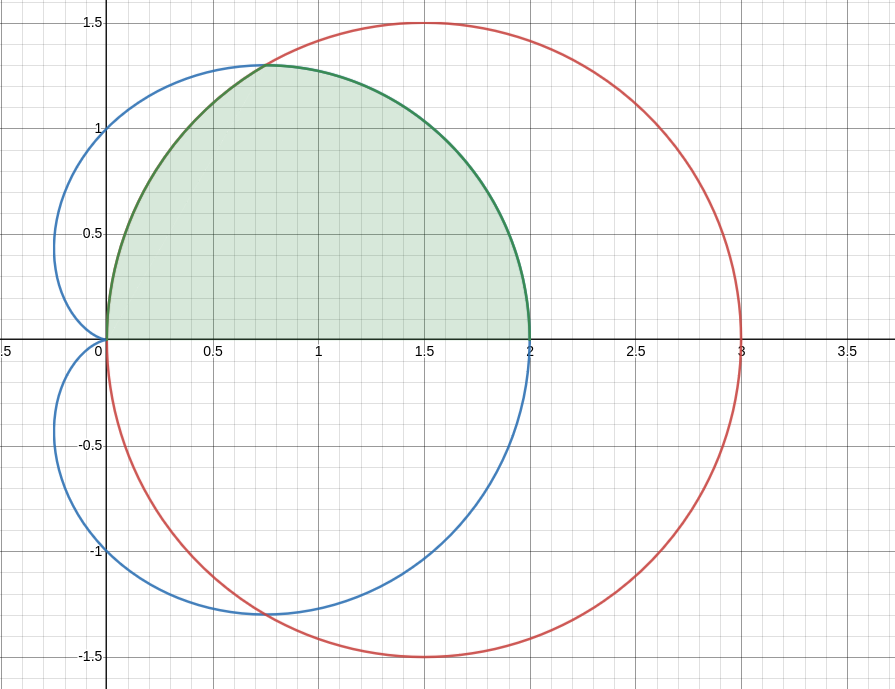
\includegraphics[scale=0.2]{exo18hw3-half.png}
		\end{center}

	The region $D_{1/2}$ will be the union of two regions $D_1$ and $D_2$, where
		\begin{align*}
		D_1 = \{ (r, \theta ) \, : \, 0 \leq \theta \leq \pi/3 , \, 0 \leq r \leq 1 + \cos \theta \}
		\end{align*} 
	and
		\begin{align*}
		D_2 = \{ (r, \theta ) \, : \, \pi/3 \leq \theta \leq \pi/2 , \, 0 \leq r \leq 3\cos \theta \} .
		\end{align*}
	See the picture below:
		\begin{center}
		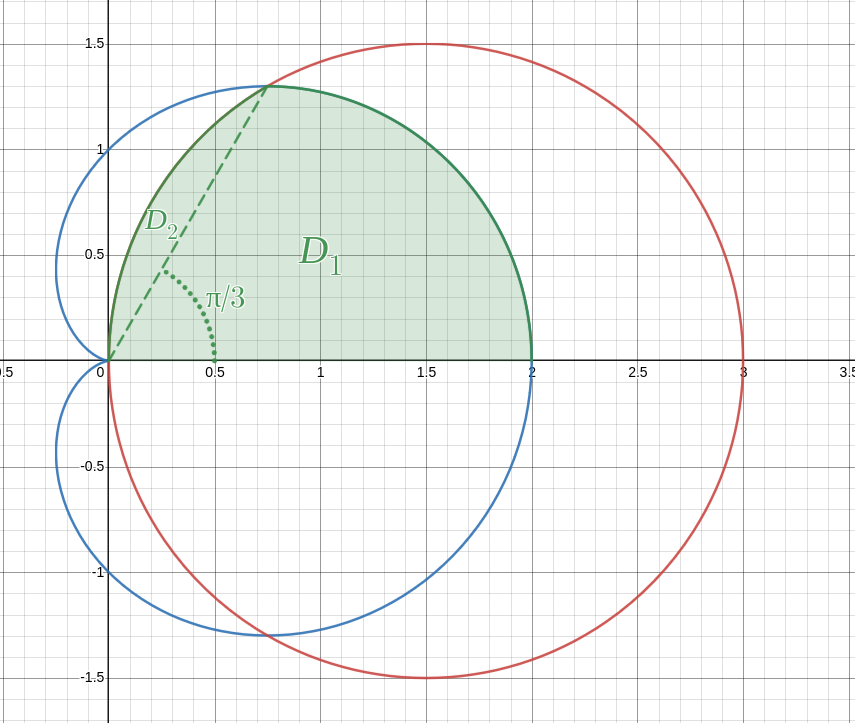
\includegraphics[scale=0.1825]{exo18hw3-sep.png}
		\end{center}
	Therefore, 
		\begin{align*}
		Area(D_{1/2}) &= Area(D_1) + Area (D_2) \\
		&= \iint_{D_1} \, dA + \iint_{D_2} \, dA \\
		&= \int_0^{\pi/3} \int_0^{1 + \cos \theta} r \, dr d\theta + \int_{\pi/3}^{\pi/2} \int_0^{3\cos \theta} r \, dr d \theta \\
		&= \int_0^{\pi/3} \frac{(1 + \cos \theta )^2}{2} \, d \theta + \int_{\pi/3}^{\pi/2} \frac{9 \cos^2 (\theta )}{2} \, d\theta \\
		&= \frac{1}{16} \Big( 9 \sqrt{3} + 4 \pi \Big) + \frac{9}{24} \Big( 2\pi - 3 \sqrt{3} \Big) \\
		&= \frac{1}{16} \Big( 16\pi - 9 \sqrt{3} \Big) \approx 2.1673 . \tag*{$\triangle$}
		\end{align*} 
	\end{comment}

	In fact, the problem asked to find the area inside the cardioid and outside the circle. By symmetry, we can restrict ourselves to the part of the region above the $x$-axis (see the picture below).
	\begin{center}
		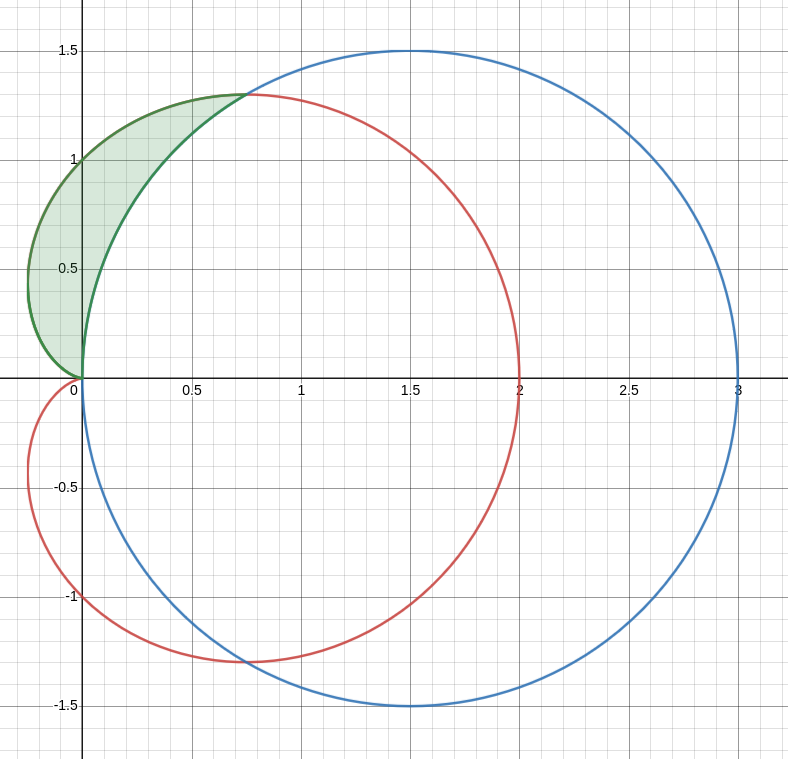
\includegraphics[scale=0.3]{exo18_15-3.png}
	\end{center}
	There will be two regions, a region $R_1$ from $\theta = \pi/3$ to $\theta = \pi / 2$ and another region $R_2$ from $\theta = \pi /2$ to $\theta = \pi$. We explicitly have
		\begin{align*}
		R_1 = \{ (r, \theta ) \, : \, 3 \cos \theta \leq r \leq 1 + \cos \theta , \, \pi/3 \leq \theta \leq \pi / 2 \}
		\end{align*} 
	and
		\begin{align*}
		R_2 = \{ (r, \theta ) \, : \, 0 \leq r \leq 1 + \cos \theta , \, \pi / 2 \leq \theta \leq \pi \} .
		\end{align*} 
	Therefore, we obtain
		\begin{align*}
		Area (R) &= 2 \Big( \iint_{R_1} \, dA + \iint_{R_2} \, dA \Big) \\ 
		&= 2 \Big( \int_{\pi / 3}^{\pi /2} \int_{3 \cos \theta}^{1 + \cos \theta} \, r dr d\theta + \int_{\pi/2}^{\pi} \int_{0}^{1 + \cos \theta} \, r dr d\theta \Big) \\ 
		&= 2 \Big( 1 - \frac{\pi}{4} + \frac{3\pi}{8} - 1 \Big) = \frac{\pi}{4} . \tag*{$\triangle$}
		\end{align*} 

	\exo{15.3}{20}{10}

	The function is $f (x, y) = \sqrt{x^2 + y^2}$ and therefore, the volume of the solid is given by
		\begin{align*}
		\mathrm{Vol} (S) = \iint_D \sqrt{x^2 + y^2} \, dA ,
		\end{align*} 
	where $D$ is the region over which is the integration. 

	The region $D$ is between two circles (an annulus):
		\begin{align*}
		D = \{ (x, y) \, : \, 1 \leq x^2 + y^2 \leq 4 \}
		\end{align*} 
	which can be described in polar coordinates, with $r = \sqrt{x^2 + y^2}$ as
		\begin{align*}
		D = \{ (r, \theta ) \, ; \, 1 \leq r \leq 2 , \, 0 \leq \theta \leq 2\pi \} .
		\end{align*} 

	So
		\begin{align*}
		\mathrm{Vol} (S) &= \int_0^{2\pi} \int_1^2 r^2 \, dr d\theta \\
		&= \Big( \int_0^{2\pi} \, d\theta \Big) \Big( \int_1^2 r^2 \, dr \Big) = \frac{14}{3} \pi . \tag*{$\triangle$} 
		\end{align*} .


	\exo{15.3}{32}{10}

	From the bounds in the integrals, we see that
		\begin{align*}
		D = \{ (x, y) \, : \, 0 \leq x \leq 2 , \, 0 \leq y \leq \sqrt{2x - x^2} \} .
		\end{align*}
	The upper bound $y = \sqrt{2x - x^2}$ can be rewritten as
		\begin{align*}
		y^2 = 2x - x^2 \iff x^2 - 2x + y^2 = 0 \iff (x - 1)^2 + y^2 = 1 .
		\end{align*} 
	So this is a circle centered at $(1, 0)$ of radius $1$. Therefore, the region $D$ is the upper half region enclosed by this circle. 

	Letting $x = r \cos \theta$ and $y = r \sin \theta$, we see that
		\begin{align*}
		y^2 = 2x - x^2 \Rightarrow r^2 \sin^2 (\theta) = 2r \cos \theta - r^2 \cos^2 (\theta ) \Rightarrow r^2 = 2r \cos \theta \Rightarrow r = 2 \cos \theta .
		\end{align*} 
	This circle intersects the $x$ axis at $x = 0$ and $x = 2$. When $x = 0$, we obtain $\theta = \pi/2$ and when $x = 2$, we obtain $\theta = 0$. Therefore,
		\begin{align*}
		\int_0^2 \int_0^{\sqrt{2x - x^2}} \sqrt{x^2 + y^2} \, dy dx &= \iint_D \sqrt{x^2 + y^2} \, dA \\
		&= \int_0^{\pi/2} \int_0^{2 \cos \theta} r^2 \, dr d\theta \\
		&= \int_0^{\pi/2} \frac{8\cos^3 (\theta )}{3} \, d\theta \\
		&= \int_0^{\pi/2} \frac{8}{3} \Big( \cos \theta - \sin^2(\theta ) \cos \theta \Big) \, d\theta \\
		&= \frac{8}{3} \left. \Big( \sin \theta \Big) \right|_0^{\pi/2} - \frac{8}{3} \int_0^1 u^2 \, du \\
		&= \frac{8}{3} - \frac{8}{9} = \frac{16}{9} .
		\end{align*} 


\end{document}